\documentclass[tikz, 11pt, margin=0.1cm]{standalone}

\usepackage{stix2}

\begin{document}
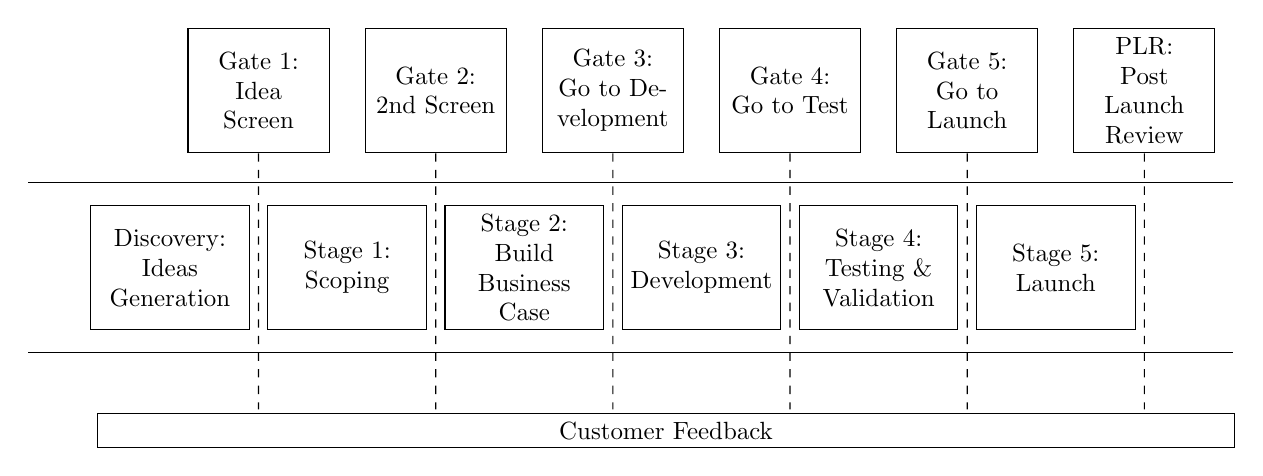
\begin{tikzpicture}[scale=0.9, every node/.style={scale=0.9}]
    \node[draw, text width=57, align=center, minimum height=50] (A) at (0,0) {Discovery:\\ Ideas\\ Generation};
    \node[draw, text width=57, align=center, minimum height=50] (B) at (2.5,0) {Stage 1:\\ Scoping};
    \node[draw, text width=57, align=center, minimum height=50] (C) at (5,0) {Stage 2:\\ Build\\ Business\\ Case};
    \node[draw, text width=57, align=center, minimum height=50] (D) at (7.5,0) {Stage 3:\\ Development};
    \node[draw, text width=57, align=center, minimum height=50] (E) at (10,0) {Stage 4:\\ Testing \&\\ Validation};
    \node[draw, text width=57, align=center, minimum height=50] (F) at (12.5,0) {Stage 5:\\ Launch};
    
    \draw[] (-2,1.2) -- (15,1.2);
    \draw[] (-2,-1.2) -- (15,-1.2);
    
    \node[draw, text width=50, align=center, minimum height=50] (G) at (1.25, 2.5) {Gate 1:\\ Idea Screen};
    \draw[dashed] (G) -- (1.25, -2);
    \node[draw, text width=50, align=center, minimum height=50] (H) at (3.75, 2.5) {Gate 2:\\ 2nd Screen};
    \draw[dashed] (H) -- (3.75, -2);
    \node[draw, text width=50, align=center, minimum height=50] (I) at (6.25, 2.5) {Gate 3:\\ Go to Development};
    \draw[dashed] (I) -- (6.25, -2);
    \node[draw, text width=50, align=center, minimum height=50] (J) at (8.75, 2.5) {Gate 4:\\ Go to Test};
    \draw[dashed] (J) -- (8.75, -2);
    \node[draw, text width=50, align=center, minimum height=50] (K) at (11.25, 2.5) {Gate 5:\\ Go to Launch};
    \draw[dashed] (K) -- (11.25, -2);
    \node[draw, text width=50, align=center, minimum height=50] (L) at (13.75, 2.5) {PLR:\\ Post Launch Review};
    \draw[dashed] (L) -- (13.75, -2);
    
    \node[draw, text width=450, align=center] (M) at (7,-2.3) {Customer Feedback};
\end{tikzpicture}
\end{document}